%\documentclass[12pt]{article}
\documentclass[BCOR=12mm,DIV11,titlepage,a4paper,oneside]{scrbook}
\usepackage{url}
\usepackage{hyperref}
\usepackage{scrhack}
\usepackage[ngerman]{babel}
\usepackage[utf8x]{inputenc}
\usepackage{amsmath}
\usepackage{graphicx}
\usepackage{caption}
\usepackage[colorinlistoftodos]{todonotes}
\usepackage{subcaption}
\usepackage{abstract}
\usepackage[printonlyused]{acronym}
\usepackage{pgfplots}
\usepackage{ragged2e}




% Default fixed font does not support bold face
\DeclareFixedFont{\ttb}{T1}{txtt}{bx}{n}{12} % for bold
\DeclareFixedFont{\ttm}{T1}{txtt}{m}{n}{12}  % for normal

% Custom colors
\usepackage{color}
\definecolor{deepblue}{rgb}{0,0,0.5}
\definecolor{deepred}{rgb}{0.6,0,0}
\definecolor{deepgreen}{rgb}{0,0.5,0}

\usepackage{listings}

% Python style for highlighting
\newcommand\pythonstyle{\lstset{
language=Python,
basicstyle=\ttm,
otherkeywords={self},             % Add keywords here
keywordstyle=\ttb\color{deepblue},
emph={MyClass,__init__},          % Custom highlighting
emphstyle=\ttb\color{deepred},    % Custom highlighting style
stringstyle=\color{deepgreen},
frame=tb,                         % Any extra options here
showstringspaces=false            % 
}}


% Python environment
\lstnewenvironment{python}[1][]
{
\pythonstyle
\lstset{#1}
}
{}

% Python for external files
\newcommand\pythonexternal[2][]{{
\pythonstyle
\lstinputlisting[#1]{#2}}}

% Python for inline
\newcommand\pythoninline[1]{{\pythonstyle\lstinline!#1!}}


%fancyheadings funktioniert nicht mehr mit der KOMA Script Klasse scrbook

\usepackage{wrapfig}

\usepackage[authoryear,round]{natbib}

% Mittels [H] können Bilder genau an einer Stelle positioniert werden
\usepackage{float}

%\usepackage[breaklinks]{hyperref}

% bewirkt das HyperLinks in der PDF nicht umrandet oder farbig sind
\hypersetup{colorlinks=false}

% package for colored text
% black,white,green,red,blue,yellow,cyan,magenta
\usepackage{color}

% package for colored tables
\usepackage{colortbl}

%Paket zur Erzeugung von Anführungszeichen durch \enquote{Text}
\usepackage[ngerman]{babel}
\usepackage[babel, german=quotes]{csquotes}

%Verhindern, dass eine neue Seite für ein einzelnes Wort/Zeile verwendet wird
\clubpenalty = 10000 % schliesst Schusterjungen aus 
\widowpenalty = 10000 % schliesst Hurenkinder aus (keine Beleidigung, sondern wirklich ein Fachbegriff)

\usepackage{lipsum}

\begin{document}
\pagenumbering{gobble}
%!TEX root = ../main.tex
\begin{titlepage}

\begin{center}

% Logo der Technische Hochschule Köln
% Kann auch in dieser Form in Schwarz/Weiß ausgedruckt werden; Graustufen sollten der .tif Version entsprechen
\begin{figure}[!ht]
%	\centering
		
\includegraphics[width=0.26\textwidth]{images/THlogoheader.pdf}
\end{figure}

\vspace{0.4cm}

%Deutscher Titel
\begin{rmfamily}
\begin{huge}
\textbf{Smart Home Interior - }\\	
\end{huge}
\vspace{0.5cm}
\begin{LARGE}
 Erkennung von Interaktionen mit einem Sofa\\ auf Basis eines neuronalen Netzes\\
\end{LARGE}
\end{rmfamily}

\vspace{0.8cm}

%Englischer Titel
% \begin{rmfamily}
% \textbf{\LARGE Title in English}\\
% \large with a very\\long subtitle\\
% \normalsize
% \end{rmfamily}

% \vspace{1.2cm}

%Bachelorarbeit 
\begin{LARGE}
\begin{scshape}
Bachelorarbeit\\[0.8em]
\end{scshape}
\end{LARGE}

%ausgearbeitet von...
\begin{large}
ausgearbeitet von\\ 
\vspace{0.3cm}
\begin{LARGE}
Jan Schröder\\
\end{LARGE}
\end{large}

\vspace{1.2cm}

%zur Erlangung des akademischen Grades...
\begin{large}
zur Erlangung des akademischen Grades\\
\vspace{0.1cm}
\textsc{Bachelor of Science (B.Sc.)}\\ 
\end{large}

\vspace{0.6cm}

%vorgelegt an der...
\begin{large}
vorgelegt an der\\ 
\vspace{0.2cm}
\begin{scshape}
Technischen Hochschule Köln\\
Campus Gummersbach\\
Fakultät für Informatik und\\
Ingenieurwissenschaften\\
\end{scshape}
\end{large}

\vspace{0.6cm}

%im Studiengang...
\begin{large}
im Studiengang\\ 
\vspace{0.1cm}
\textsc{Informatik}
\end{large}


\vspace{1.2cm}

%Autor der Bachelorarbeit und die Prüfer
\begin{tabular}{rl}
        Erster Prüfer/in:  &  Prof. Dr. Matthias Böhmer\\
       					&  \small Technische Hochschule Köln \\[1.0em]
       Zweiter Prüfer/in:  &  Prof. Dr. rer. nat. Wolfgang Konen\\
       					&  \small Technische Hochschule Köln\\
\end{tabular}

\vspace{1.2cm}

%Ort, Monat der Abgabe
\begin{large}
Gummersbach, \today
\end{large}

\end{center}

\newpage
\thispagestyle{empty}

%Kontaktmöglichkeiten des Autors und der Prüfer
\begin{center}
\begin{tabular}{rl}
							&  \\[26.0em]
							
\large \textbf{Adressen:}	&  	\quad Jan Schröder\\
							&  	\quad Wilhemlstr. 12\\
							&	\quad 51643 Gummersbach\\
							&  	\quad jan.schroeder1@smail.th-koeln.de\\[2.0em]
							
							&  	\quad Prof. Dr. Matthias Böhmer\\
							&  	\quad Technische Hochschule Köln\\
							&  	\quad Institut für Informatik\\
							&	\quad Steinmüllerallee 1\\
							&	\quad 51643 Gummersbach\\
							&  	\quad matthias.boehmer@th-koeln.de\\[2.0em]
							
							&  	\quad Prof. Dr. rer. nat. Wolfgang Konen\\
							&  	\quad Technische Hochschule Köln\\
							&  	\quad Institut für Informatik\\
							&	\quad Steinmüllerallee 1\\
							&	\quad 51643 Gummersbach\\
							&  	\quad wolfgang.konen@th-koeln.de\\[2.0em]
\end{tabular}
\end{center}

\end{titlepage}


\tableofcontents
\newpage

\pagenumbering{arabic}
\chapter*{Vorwort zum Aufbau der Bachelorarbeit}
Die Arbeit gliedert sich in sechs Teile. Der erste Teil widmet sich der Einleitung und einem Einblick in den Inhalt. Daraufhin werden im zweiten Teil die Grundlagen behandelt. Diese sollen ein Verständnis vermitteln, um die weiteren Kapitel der Bachelorarbeit zu verstehen. 
\newline
\newline
Anschließend behandelt der Autor im dritten Teil der Arbeit die Architektur des Prototypen, welcher in der Bachelorarbeit benutzt wird. Zusätzlich behandelt dieser Teil die Architektur des Prototypen aus dem Praxisprojekt um die späteren Veränderungen zu veranschaulichen. Dies ist notwendig, da der Autor die Veränderungen in den weiteren Teilen der Bachelorarbeit beschreibt.
\newline
Auf der Grundlage aus dem zweiten Teil der Arbeit wird die Umsetzung des neuronalen Netzes im vierten Teil beschrieben. Außerdem wird ein Vergleich aus dem Regelsystem gezogen, welches im Rahmen des Praxisprojekts entwickelt wurde.
\newline
Weiterhin beschreibt das fünfte Kapitel die Evaluation aus der Sammlung der Trainingsdaten und der Ergebnisse aus dem neuronalen Netz.
\newline
\newline
Abschließend findet im sechsten Teil ein Fazit statt, welches die Endergebnisse der Arbeit veranschaulicht und wie der Prototyp in Zukunft weiterentwickelt werden kann.
Als Anhang findet man Teile aus dem Programmcode der Programme, die für die Bachelorarbeit geschrieben wurden.
\newpage
\chapter*{Abstract}
Diese Bachelorarbeit behandelt ein System bestehend aus Sensoren, welche mit einem ESP32 und Raspberry Pi einen Sofaprototypen bilden. Der Prototyp zur Sammlung der Sensorwerte und ein neuronales Netz sind die beiden Kernkomponenten. Der aktuelle Prototyp hat Ultrasonic-Sensoren angeschlossen, welche zur Messung der Rückenlehne benutzt werden. Dieser Sensor ist nicht geeignet, da dieser zu auffällig ist und nur im Radius vor der Rückenlehne messen kann. Daher sollte dieser durch einen FSR-Sensor ersetzt werden. Das neuronale Netz kann noch nicht zu 100\% Vorhersagen treffen, kommt mit einer Vorhersage von 99,7\% aber schon nah dran. Diese Vorhersage tritt nur bei dem Datensatz auf, der alle Datenpunkte beinhaltet. Es ist also wichtig, dass der Input für das neuronale Netz so nah wie möglich an der Realität ist.

\newpage
\chapter{Einleitung}
\label{cha:Einleitung}

\section{Motivation und Relevanz zum Thema Smart Home Interior}

\section{Idee zur Umsetzung vom Regelsystem zum neuronalen Netz}

\section{Personen an die das System gerichtet ist}

\section{Ziel der Bachelorarbeit}
\newpage
%!TEX root = ../VorlageBA.tex
\chapter{Grundlagen aus dem IoT für das Thema Smart Home Interior}
\label{cha:grdl}

\addtocontents{toc}{\protect\setcounter{tocdepth}{1}}
\section{Smart Home Aufbau und Funktion}
Ein Smart Home ist ein System, welches automatisch smarte Geräte im Haus steuert. Die smarten Geräte können aber auch zusätzlich durch den Nutzer im Haus gesteuert werden. Dies ist durch verschiedene Kommunikationsmethoden möglich. Diese Kommunikation kann z.B. durch Bluetooth, WiFi oder auch Infrarot durch den Nutzer oder der Smart Home Automatisierung geschehen. Ein smartes Gerät ist ein Gerät, welches mit einem Computer ausgestattet ist und damit die Funktionalität des Gerätes erweitert. Für den Prototypen der Bachelorarbeit wird ein wireless System verwendet. Über das MQTT Protokoll werden die Daten im Netzwerk versendet. Näher erläutert wird dies in Kapitel \ref{cha:arch_pro}. 
\newline
Durch die Automatisierung ist es also möglich, dass bestimmte Interaktionen im Haus nicht mehr manuell vom Bewohner des Hauses getätigt wird. Für jeden Raum wird in der Regel eine unterschiedliche Automatisierung erstellt, da zu unterschiedlichen Zeiten andere smarte Geräte im Raum aktiviert werden. Da im Haus oft Geräte Strom verbrauchen, dabei aber nicht benutzt werden, kann ein Smart Home die smarten Geräte auch so verwalten, dass sie nur dann Strom verbrauchen, wenn sie auch wirklich vom Nutzer aktiv verwendet werden. Sollte das nicht passieren, kann das Smart Home den Stromkreis automatisch unterbrechen. Zusätzlich können damit auch gefährliche Situationen vermieden werden. \citep{sripan2012research}
\newline
Mit den genannten Funktionen ist es möglich verschiedene Smart Home Systeme zu entwickeln. So haben Personen die ohne Hilfe ihren Alltag nicht mehr bewältigen können oder Personen die medizinische Unterstützung brauchen die Möglichkeit, trotzdem selbstständig zu leben. 

\subsection{Neuronale Netze in Smart Homes}
Ein neuronales Netz ist in der Lage das Verhalten von Menschen zu erkennen um so in Smart Homes unter anderem das Strom Management zu verbessern. Anhand von Sensoren wird dann gemessen, unter anderem wie viele Personen sich im Raum befinden und was sie damit wirklich an Strom brauchen. Anhand der Sensorwerte und dem Verhalten der Menschen entscheidet das neuronale Netz dann, welches Gerät ausgeschaltet werden kann. \citep{badlani2011smart} Aus dieser wissenschaftlichen Arbeit ist also zu erkennen, dass ein neuronales Netz durch Interaktionen mit Sensoren die Steuerung der smarten Geräte verwalten kann.

\section{Smart Home Interior}
Das Teilgebiet Smart Home Interior zeigt die digitalisierung der Innenausstattung in einem Smart Home. So wird gezeigt, dass die Möbel im Haus oder der Wohnung als smartes Möbelstück genutzt werden können. Sitzmöbel werden dann als Steuerung anderer smarter Möbel oder Geräte eingesetzt. Außerdem ist es dann möglich für die Möbel eine zusätzliche Automatisierung zu entwickeln und in das Smart Home mit zu integrieren. Smarte Möbel dienen zur passiven Steuerung von smarten Geräten oder Möbelstücken. Der Nutzer muss nicht mehr aktiv ein Tablet oder ähnliches Gerät erst entsperren, die App raussuchen und dann darüber steuern, sondern braucht nur noch eine aktive Interaktion mit den Möbeln haben und diese steuern ohne weiteren Einfluss der Person die Geräte. So spart der Nutzer Zeit und ist nicht mehr gestresst. 
\newline
Für das Sofa ist also nur wichtig, dass sich alle Geräte, welche gesteuert werden sollen in einem Netz befinden. Es werden keine weiteren Apps mehr gebraucht um verschiedene Geräte von verschiedenen Herstellern zu nutzen.

\section{Neuronale Netze zur Klassifizierung}
\label{sec:NNK}
Das folgende Kapitel befasst sich Grundlagen zu neuronalen Netzen. Umfasst wird dabei der Aufbau, wie die Berechnungen auf den Layern stattfinden, wie klassifiziert wird und Allgemeinbegriffe geklärt. Da das Thema zu neuronalen Netzen sehr breit ist, wird hier nur das erläutert, was der Autor auch zur Umsetzung und Evaluation in den späteren Kapiteln benutzt. So sollen später benutzte Fachbegriffe und Methoden nicht in jedem Kapitel neu erklärt werden.

\subsection{Aufbau eines neuronalen Netzes}
Ein neuronales Netz beinhaltet für die Daten der Außenwelt in Form von Zahlenwerten einen Input-Layer. Die Input-Units empfangen diese Werte. Daraufhin werden die Daten weiterverarbeitet und an die Hidden-Units im Hidden-Layer gesendet. Es können mehrere Hidden-Layer je nach Aufgabe des neuronalen Netzes existieren. Nach den Hidden-Layern kommt als letztes der Output-Layer mit den Output-Units. Der Output-Layer gibt die Zahlenwerte aus, die die Vorhersage des neuronalen Netzes als Ergebnisse auch in Form von Zahlenwerten liefern.

\subsection{Berechnung der Inputwerte}
Zwischen den einzelnen Neuronen existieren Gewichtungen  \(w_1 \dots w_n\) welche willkürlich gewählt werden. Diese werden mit den Eingabewerten  \(a_1 \dots a_n\) multipliziert. Diese Multplikationen werden als summiert. Die Aktivierungsfunktion rechnet die Ergebnisse aus dieser Summe aus.
\newline
\[\displaystyle\sum_{i=1}^{n} a_i w_i = (a_1 \cdot w_1 + a_2 \cdot w_2 + \dots + a_{n-1} \cdot w_{n-1} + a_n \cdot w_n)\]
\newline
Zu dem Layer kann dann eine Bias-Unit dazu addiert werden. Dies ist ein konstanter Wert, welcher eins beträgt. So wird die Aktivierungsfunktion später abgeändert, damit sich kein Wert überschneidet.
\newline
Ab der Hidden Schicht wird die Bias-Unit dazu genommen. Da der Input-Layer oft nicht als eigene Schicht in Programmiersprachen betrachtet wird, wird die Bias-Unit auch im neuronalen Netz des Prototypen sofort mit dazu gerechnet.

\subsection{Die Trainingsphase und Testphase mit einlesen von Testdaten}
Bei einem neuronalen Netz gibt es zwei Phasen - die Trainings- und die Testphase. Bei der Trainingsphase werden Testdaten über ein Dataset eingelesen. Dieses Dataset können entweder Vektoren oder Matrizen sein. Anhand dieses Datasets können die Gewichtungen angepasst werden, damit das neuronale Netz, dass trainierte in der Testphase anwenden kann.
\newline
Anders als in der Trainingsphase werden in der Testphase keine neuen Datasets eingelesen. Durch die angepassten Gewichte aus der Trainingsphase kann in der Testphase erkannt werden, was das neuronale Netz gelernt hat. Um zu testen, ob das neuronale Netz eine richtige Vorhersage macht, werden neue Zahlenwerte eingegeben und geprüft.

\subsection{Die sigmoid Aktivitätsfunktion zur Backpropagation}
\label{sec:inp}
Nachdem nun das Dataset eingelesen wurde und die Summe aus der Propagierungsfunktion errechnet ist, wird das Ergebnis in die Aktivitätsfunktion für die Backpropagation eingegeben. Die sigmoid Funktion ist die am häufigsten genutzte Aktivitätsfunktion. Da deren Ergebnisse zwischen null und eins liegen, wird diese Funktion auch für den Prototypen zur Klassifikation benutzt. \citep{Rey2011} Durch das genannte Intervall ensteht ein höheres Spektrum von Möglichkeiten zur Klassifizierung. Anders als bei der step Funktion werden die Ergebnisse größer null mit dem Ergebnis eins ausgegeben. Alle Ergebnisse darunter werden als null ausgegeben.

\begin{tikzpicture}
    \begin{axis}[
    	legend pos=north west,
        axis x line=middle,
        axis y line=middle,
        x tick label style={/pgf/number format/fixed,
                            /pgf/number format/fixed zerofill,
                            /pgf/number format/precision=1},
        y tick label style={/pgf/number format/fixed,
                            /pgf/number format/fixed zerofill,
                            /pgf/number format/precision=1},
        grid = major,
        width=11cm,
        height=7cm,
        grid style={dashed, gray!30},
        xmin=-1,     % start the diagram at this x-coordinate
        xmax= 1,    % end   the diagram at this x-coordinate
        ymin= 0,     % start the diagram at this y-coordinate
        ymax= 1,   % end   the diagram at this y-coordinate
        %axis background/.style={fill=white},
        xlabel=x,
        ylabel=y,
        tick align=outside,
        enlargelimits=false]
      % plot the stirling-formula
      \addplot[domain=-1:1, blue, ultra thick,samples=500] {1/(1+exp(-10*x))};
      \addlegendentry{$g(x)=\frac{1}{1+e^{-x}}$}
    \end{axis}
\end{tikzpicture}

\subsection{Backpropagation}
Bei der Backpropagation läuft das neuronale Netz nochmal rückwärts ab um die Gewichte so zu verändern, dass die Fehler auf ein minimum reduziert werden. Wie schon in Kapitel \ref{sec:inp} genannt, wird die sigmoid Funktion verwendet. Wenn aus der sigmoid Funktion die Ergebnisse ausgegeben werden, werden diese an die abgeleitete sigmoid Funktion geschickt. Durch diese abgeleitete Funktion zeigen die Ausgabewerte aus dem feed forward Schritt, wie stark die Gewichtungen abweichen um das gewünschte Ergebnis zu erreichen.
\newline
So wird bei der Backpropagation ein Neuron in zwei Teile aufgeteilt. Auf der rechten Seite ist die Aktivierungsfunktion und auf der linken Seite deren Ableitung. 

\subsection{Ausgabe der Ergebnisse als Klassifizierung}
Das neuronale Netz des Prototypen arbeitet mit der Vorhersage, die Endergebnisse richtig oder falsch zu klassifizieren. In einem zweidimensionalen Diagramm sind die Ergebnisse als x und y Werte im Diagramm dargestellt. Abbildung \ref{fig:nn_class} zeigt ein solches Diagramm mit drei Klassen. Die Punkte stellen die gewünschten Ergebnisse in der richtigen Klasse dar.

\begin{figure}[H]
	\centering
		%[natürliche Breite in Pixeln, natürliche Höhe in Pixeln, Abhängigkeit von der Textbreite]
		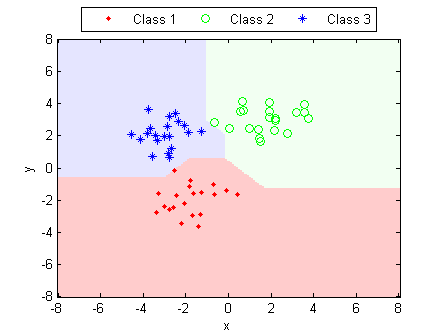
\includegraphics[width=0.75\textwidth]{images/nn_classifier.png}
	\caption{Beispiel eines classifiers}
	\label{fig:nn_class}
\end{figure}

Um die Ergebnisse richtig zu klassifzieren, müssen die korrekten Klassifizierungen in die Richtung des Wertes eins gehen und alle anderen Ergebnisse Richtung null. Daher ist wieder zu erwähnen, dass die sigmoid Funktion für dieses neuronale Netz geeignet ist.

\section{MQTT zur Datenübertragung}
MQTT ist ein Protokoll, welches mit der Publish/Subscribe Methode arbeitet. Mikrocontroller und Sensoren publishen ihre Daten an den MQTT Broker. Der Broker speichert diese Daten bis Subscriber diese Nachrichten zugesendet bekommen. Jeder Subscriber bekommt diese Nachrichten dann gleichzeitig. Diese Clients können ihre Daten wiederum auch publishen und wieder an neue Geräte die Subscriber sind versenden. Als Clients sind intelligente Geräte gemeint wie Mikrocontroller oder PCs. Publisher versenden also Nachrichten und Subscriber erhalten diese. Also kann ein Client sowohl Publisher als auch Subscriber sein. \citep{soni2017survey} Für die Kommunikation ist demnach ein TCP-Stack und das MQTT-Protokoll vorausgesetzt. Zusätzlich ist eine Verbindung zum MQTT-Broker erforderlich wo der Typ des Netzes aber unwichtig ist. Die Anzahl der Clients die aktiv als Subscriber oder Publisher dienen ist nicht relevant. Wichtig ist dabei nur, dass der Broker funktioniert und Verfügbar für die Clients ist. Außerdem ist zu erwähnen, dass es nicht relevant ist, dass sowohl Publisher als auch Subscriber gleichzeitig aktiv sein müssen. Der Broker kann die Nachrichten auch dann noch übermitteln, auch wenn der Publisher nicht mehr aktiv ist. Damit Nachrichten versendet werden, gibt es die topics. Dabei ist es nicht wichtig, über welche Struktur die Nachricht aufgebaut ist. \citep{Trojan2017}
\newline
MQTT ist mit dieser Methode also ein Protokoll, was passend für diesen Prototypen ist, da es für das Senden von Sensordaten in einem Wireless Network ausgelegt ist. Der Mosquitto Broker findet in diesem System Verwendung zur Nachrichtenübermittlung. 
\newline
\newline
Das Protokoll hat drei Stufen des Quality of Service. Diese werden in der Tabelle \ref{tab:tableqos} dargestellt. Die Stufen dienen zur Sicherung der Nachrichtenübermittlung auch wenn das Netz Störungen beim übertragen hat.

\begin{table}[ht]
	\centering
	\caption[Tabellarische Darstellung der QoS Level]{Tabellarische Darstellung der QoS Level \citep{soni2017survey}}
		\vspace{1.0em}	
	\begin{tabular}{| l | l | p{5cm}|}
		\hline
		\rowcolor[gray]{0.9}\textbf{Stufen} & \textbf{Häufigkeit} & \textbf{Beschreibung} \\
		\hline
		\hline
		0 & höchstens eine Nachricht & Es wird maximal eine Nachricht versendet, ohne eine Garantie, dass diese auch ankommt \\
		\hline
		1 & mindestens eine Nachricht & Es ist möglich, dass eine Nachricht mehr als einmal versendet wird\\
		\hline
		2 & genau eine Nachricht & Eine Nachricht wird mit einem Four-Way Handshake versendet\\
		\hline
	\end{tabular}
	\label{tab:tableqos}
\end{table}

\section{Sensoren für die Interaktionen auf dem Sofa}
\subsection{Erläuterung des Raspberry Pi 3 und des ESP32}
Der Raspberry Pi 3 ist ein Einplatinen Computer, auf dem das Betriebssystem Raspbian installiert ist. Das Betriebssystem basiert auf Linux Debian und läuft in der aktuellen Version 10 - Buster. Neben den Möglichkeiten den Raspberry Pi für einfachere Anwendungen zu Verwenden ist es auch möglich, verschiedene Sensoren an dessen GPIO Pins anzuschließen. Der Raspberry Pi 3 hat einen eine interne WiFi Karte und kann damit in einem WLAN Netzwerk eingebunden werden. Dies wird gebraucht, da der Prototyp in einem lokalen Netzwerk ausgeführt wird.
\newline
Der ESP32 ist ein Mikrocontroller, welcher als Nachfolger vom ESP8266 weitere GPIO Pins bekommen hat um mehr als einen Analogen Sensor anschließen zu können. Ein ESP32 hat ein Live Betriebssystem und kann nur ein Programm ausführen, welches vorher hochgeladen werden muss. 

\subsection{Sensoren die für den Prototypen verwendet werden}
Für den aktuellen Prototyp werden Ultrasonic Sensoren und Force Sensitive Resistors verwendet. 
Diese reichen aus um Sitz- und Liegepositionen der Nutzer zu erkennen. Der Ultrasonic Sensor misst anhand von Wellen den Abstand zwischen dem Sensor und einem Gegenstand.
\newline
Der FSR misst anhand des elektrischen Widerstands den Druck, welcher zwischen 100 Gramm und 10 Kilogramm beträgt. Bei allen Gewichten über zehn Kg zeigt der Sensor immer den höchsten Wert. \citep{florez2010calibration}
Sie sind aus zwei Polymer Schichten gebaut. Eine leitende Oberfläche und eine andere an die erste bindende Schicht mit Elektroden. \citep{hollinger2006evaluation} Diese Sensoren werden also dafür verwendet um zu erkennen, wann die Personen Druck auf sie einüben indem sie ihn mit ihrem Gewicht auslösen. Als FSRs werden die interlink FSR Sensoren eingesetzt.

\section{Prototyp aus dem Praxisprojekt}
Im Rahmen des Praxisprojekts entsteht ein Prototyp, welcher die Interaktionen als Regelsystem mit sieben Regeln verwaltet. Ein ESP32 misst die Sensordaten von zwei FSRs und einem Ultrasonic Sensor. Jeder Sensor wird als MQTT Client deklariert und sendet Codes die er aus den Sensordaten erstellt. Zusätzlich messen zwei ESP8266 die Daten von Flex Sensoren, welche den Widerstand durch ihre Biegung messen. Dies erwies sich aber als ein Nachteil, da die Biegung erst ab 45 Grad gemessen wird. Ein Raspberry Pi 2 führt einen MQTT Broker Service aus und kann Daten von den ESPs empfangen, die über die Publish Methode die Codes versenden. Auf dem Raspberry Pi 2 läuft zusätzlich ein Python Programm, welches die Codes als Subscriber empfängt und im Regelsystem verwaltet. Die Regeln werden als Codes neu an den MQTT Broker gepublished und können dann von jedem beliebigen Subscriber empfangen werden. \citep{Schroeder2019} 
\newline
Was bei der Nutzung des Regelsystems aber nicht beachtet wurde, sind die Ausreißer der FSR Sensorwerte. Mit dem Regelsystem zielt man darauf ab, dass die FSRs immer bei nicht benutzung den Wert null haben und wenn sie besetzt sind, den Wert 1024. Während des Tests sind diese Ausreißer immer wieder aufgefallen. Damit passiert es also, dass manchmal der FSR Sensor eine Interaktion erkennt, obwohl keine stattfindet.
Kapitel \ref{sec:ums_nn} zeigt die Lösung im neuronalen Netz und Kapitel \ref{sec:arch_sofa} stellt die Hardware Lösung im Prototypen dafür dar.
\newpage
\chapter{Architektur und Aufbau des Prototyps}
\label{cha:arch_pro}
In Kapitel \ref{cha:grdl} werden die Grundlagen zum MQTT-Protokoll und den Sensoren erklärt. Auf Basis dieser Themen wird die Architektur und der Aufbau des Prototyps im dritten Teil der Bachelorarbeit beschrieben. Des weiteren wird erklärt, welche Änderungen in der Architektur vom Prototypen des Praxisprojekts vorgenommen werden. Außerdem erklärt der Autor die Änderungen, welche beim Prototypen in der Bachelorarbeit auftreten.

\section{Anforderungen an die Architektur}
Der Einsatz eines Möbelstücks wie Sitzmöglichkeiten zur Steuerung von Interaktionen ist typischerweise an eine Umgebung gebunden. Dies bedeutet, dass bspw. ein Sofa also einen festen Platz im Raum hat und nicht bewegt wird. Damit der Nutzer den vollen Funktionsumfang dieser Steuerung nutzen kann, ist es wichtig, dass dabei die herkömmlichen Positionen auf dem Sofa als Klassifizierung angewendet werden. So muss der Anwender sich nicht an neue Positionen gewöhnen, sondern kann mit dem Sofa so interagieren, wie er es im Alltag auch ohne Steuerung würde. 
\newline
\newline
Daraus wird abgeleitet, dass die Hardware-Architektur als finale Version nicht sichtbar sein darf und der Nutzer nichts von dieser mitbekommt. Zusätzlich ist noch wichtig zu erwähnen, dass durch seine Interaktionen erkannt werden muss, welche smarten Geräte er steuern möchte. Damit das neuronale Netz entsprechend steuert, welche smarten Geräte der Nutzer mit seinen Interaktionen ausführt, muss dies über vorherige Einrichtung geschehen oder einer automatischen Erkennung, welche erkennt was der Nutzer in bestimmten Interaktionen häufig nutzt. Dies ist aber nicht Teil dieser Bacheloarbeit und wird damit auch nicht weiter behandelt. Wenn diese Interaktionen erfolgreich klassifiziert werden, muss das neuronale Netz mit in das System eingebunden werden. 
\newline
In der Abbildung \ref{fig:arch_grob} wird der Aufbau des Systems gezeigt und wie dieser Ablauf stattfinden soll. Der Prototyp umfasst die Aufnahme der Interaktionen und deren Verarbeitung von drei Positionen im neuronalen Netz. Kapitel \ref{sec:ums_nn} beschreibt die Umsetzung dieses neuronalen Netzes.

\begin{figure}[H]
	\centering
		%[natürliche Breite in Pixeln, natürliche Höhe in Pixeln, Abhängigkeit von der Textbreite]
		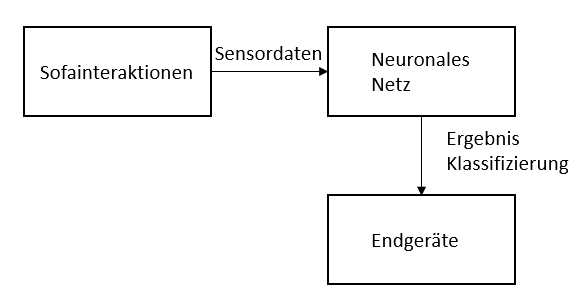
\includegraphics[width=0.6\textwidth]{images/arch_grob.png}
	\caption{Visuelle Darstellung zum Aufbau des Systems}
	\label{fig:arch_grob}
\end{figure}


\section{Architektur des Sofaprototypen aus dem Praxisprojekt}
\label{sec:arch_pp}
Der Prototyp ist ein im Rahmen des Praxisprojekts entwickeltes System, welches als verteilte Architektur aufgebaut ist. Während der Bachelorarbeit wird der Prototyp weiter ausgearbeitet und für die weiteren Versuche so optimiert, wie es in Kapitel \ref{sec:arch_sofa} erläutert ist. In diesem Kapitel wird nur die Version aus dem Praxisprojekt zum Vergleich der aktuellen Version des Prototyps während der Bachelorarbeit erläutert.
\newline
\newline
Ein ESP32 misst die Sensordaten eines Ultrasonic-Sensors sowie eines FSR-Sensors. Zwei Flex-Sensoren sind separat an jeweils einem ESP8266 angeschlossen. So bietet der Prototyp nur die Möglichkeit für eine Person zu sitzen oder auf den Sitzflächen mit den Flex-Sensoren zu liegen. Diese Daten schicken sie an einen Raspberry Pi 2, welcher diese an ein Regelsystem weitergibt, dessen Regeln in \ref{sec:rules} aufgeführt sind. Das Regelsystem ist in dieser Version des Prototypen die Hauptkomponenten, um die Interaktionen zu verwalten. Die verarbeiteten Daten, welche über \emph{if-Abfragen} in Regeln umgewandelt sind, werden über den Broker an die smarten Geräte gesendet. In diesem Prototyp sind noch keine smarten Geräte integriert, da diese Einbindung kein primäres Ziel ist. Mit diesem Prototypen ist es möglich, dass Personen mit festen Interaktionen die smarten Geräte steuern ohne, dass der Nutzer Einfluss auf diesen Vorgang nimmt. Damit sind die Interaktionen davon abhängig, wie der Nutzer mit dem Sofa interagiert. Werden die Sensoren in einer anderen Art und Weise verwendet wie es nicht vom Regelsystem vorgesehen ist, so können die erwünschten smarten Geräte nicht gesteuert werden. Somit ist das Regelsystem ein erheblicher Nachteil für Personen, die das Sofa zum ersten Mal benutzen oder für Personen, welche körperlich oder geistig benachteiligt sind sowie Personen sehr hohen Alters.
\newline
Unter anderem wird aus diesem Grund auch das neuronale Netz entwickelt und ersetzt damit das Regelsystem. Zusätzlich werden die Flex-Sensoren nicht mehr für die Liegepositionen benötigt, da diese nicht dafür geeignet sind. Um die Liegeposition dennoch zu erkennen, übernehmen die Kombinationen der Drucksensoren auf den Sitzkissen diese Aufgabe. Es ist wichtig zu erwähnen, dass die Architektur aus dem Praxisprojekt so ausgelegt ist, dass nur eine Person auf einem Platz sitzen kann und die anderen Sitzkissen nur mit Flex-Sensoren verbaut sind. Auf den nicht besetzten Plätzen ist es jedoch nicht möglich, dass andere Personen dort zusätzlich Platz nehmen. 

\section{Die Anpassung der Architektur für das neuronale Netz}
\label{sec:arch_sofa}
Dieses Kapitel beschreibt die Architektur der Bachelorarbeit und zeigt die Unterschiede aus Kapitel \ref{sec:arch_pp} zur aktuellen Architektur. Kapitel \ref{sec:komm} beschreibt die Kommunikation mit MQTT, weshalb dies auch in diesem Kapitel nicht weiter erläutert wird.

\begin{figure}[H]
	\centering
		%[natürliche Breite in Pixeln, natürliche Höhe in Pixeln, Abhängigkeit von der Textbreite]
		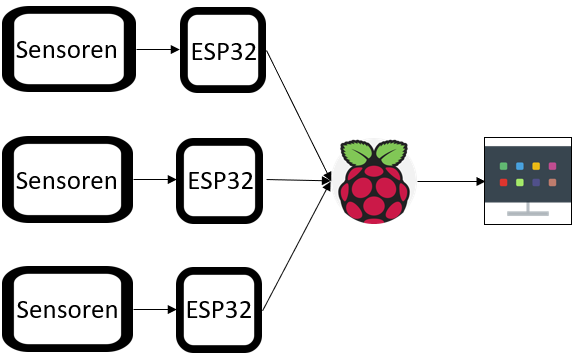
\includegraphics[width=0.6\textwidth]{images/Architektur.png}
	\caption{Abschließende Architektur mit einem Endgerät als Beispiel}
	\label{fig:arch}
\end{figure}

Abbildung \ref{fig:arch} zeigt die Architektur des überarbeiteten Prototypen. Als Sensoren werden Ultrasonic-Sensoren und Force Sensitive Resistores benutzt. Die Ultrasonic-Sensoren messen den Abstand um zu erkennen ob eine Person angelehnt ist. Die FSR-Sensoren messen anhand des Drucks ob eine Person sitzt, liegt oder mit den Armlehnen interagiert. Da dieser Prototyp für ein drei Personen Sofa ausgelegt ist, haben die beiden äußeren ESPs auch jeweils einen FSR für die Armlehnen angeschlossen. Der Raspberry Pi übernimmt die Aufgabe des MQTT-Brokers und der Aufnahme und Weitergabe der Sensorwerte. Der hier dargestellte Fernseher ist ein Beispiel für ein smartes Endgerät. Powerbanks sorgen für die Stromversorgung der Mikrocontroller und des Raspberry Pis. Alternativ ist auch das Anschließen eines Stecker für Steckdosen möglich. Als nächstes ist wichtig zu klären, ob der Prototyp als Cloud-Architektur oder lokales Netzwerk benutzt wird.
\newline
Hinsichtlich dieser Architektur reicht für das System ein lokales Netzwerk aus. Im Vergleich zu einer Cloud-Architektur ist es nicht möglich von außen auf das System zuzugreifen. Da die Steuerung sich nur innerhalb des Smart Homes befindet, reicht das lokale Netzwerk dafür aus. Eine Cloud-Architektur ergibt also nur Sinn, wenn Nutzer außerhalb des im Smart Homes auf die Geräte zugreifen wollen. Das kann der Nutzer aber nicht, da das Sofa sich immer innerhalb des Smart Homes befindet. 

\newpage

\section{Regelsystem zur Steuerung der Interaktionen} 
\label{sec:rules}
Das neuronale Netz ersetzt in der aktuellen Version des Prototypen das Regelsystem. Das Regelsystem ist ein statisches System, welches feste Regeln beinhaltet. Dieses wird in diesem Abschnitt näher erläutert. Es sollen Vor- und Nachteile veranschaulicht werden und weshalb es durch das neuronale Netz ersetzt wird.
\newline
Das Regelsystem ist so ausgelegt, dass je nach Verwendung der Sensoren eine Regel bzw. ein Code erstellt wird. Der Nachteil dieses Systems ist der statische Aufbau. Wenn eine Regel ausgelöst wird, muss jeder Benutzer immer die gleichen Sensoren auslösen um eine Regel zu nutzen. So muss bei einer Erweiterung mit neuen Regeln der Python-Code immer angepasst werden. Das hat den Nachteil für Menschen, die das System nicht kennen und zum ersten Mal benutzen. Vor allem müssen sie den Code selbst erweitern.
\newline
Da sich jede Person anders hinsetzen kann, aber das gleiche Gerät steuern möchte, kann dies nicht vom Regelsystem erkannt werden. Daher hat der Autor die Architektur und damit auch die Weiterführung des Prototypen ersetzt. Die Tabelle \ref{tab:tablerules} beschreibt dennoch noch einmal die Regeln und welche Kombination von Sensoren ausgelöst werden muss, damit man die Regeln an ein smartes Gerät sendet. Die Aufzählungen der Regeln sind auch gleichzeitig die Codes, die gepublished werden, um die smarten Geräte zu steuern. 
\newline
Mit dem Regelsystem gibt es drei FSR-Sensoren und einen Ultrasonic-Sensor für die Sitzpositionen im Prototypen. Für die Liegeposition werden zwei Flex-Sensoren benutzt. Die Flex-Sensoren fallen mit dem einsetzen des neuronalen Netzes weg, da auf den entsprechenden Plätzen andere Sensoren verwendet werden. Dies passiert, weil die Sensoren eine Biegung von mindestens 45 Grad brauchen, damit sie erkennen, dass jemand auf ihnen liegt. Daher werden nun FSR-Sensoren für die Liegepositionen eingebaut. Diese erkennen, ob eine Person sitzt oder liegt. Somit müssen dann nicht mehr zwei Sensoren in die Sitzkissen eingebaut werden. Das positive an diesem Regelsystem ist die Erweiterbarkeit der Regeln für den Entwickler. Dabei wird im Programm nur die neue Regel mit einer \emph{if-Abfrage} erweitert.

\begin{table}[H]
	\centering
	\caption[Aufzählung der Regeln des Regelsystems]{Aufzählung der Regeln des Regelsystems}
		\vspace{1.0em}	
	\begin{tabular}{|l|p{7cm}|}
		\hline
		\rowcolor[gray]{0.9}\textbf{Regeln} & \textbf{Beschreibung} \\
		\hline
		\hline
		1 & Alle FSR-Sensoren und der Ultrasonic-Sensor messen Daten \\
		\hline
		2 & Nur der FSR-Sensor auf dem Sitzkissen misst Daten
		    und der Ultrasonic-Sensor \\
		\hline
		3 & Beide FSR-Sensoren messen Daten \\
		\hline
		4 & Der FSR-Sensor auf dem Sitzkissen misst Daten \\
		\hline
		5 & Der FSR-Sensor auf dem Sitzkissen und die beiden Flex-Sensoren messen Daten \\
		\hline
		6 & Beide Flex-Sensoren messen Sensordaten \\
		\hline
		7 & Ein Flex-Sensor und der FSR-Sensor auf dem Sitzkissen messen Daten \\
		\hline
	\end{tabular}
	\label{tab:tablerules}
\end{table}

\section{Verarbeitung der Daten im ESP und Raspberry Pi}
Kapitel \ref{sec:arch_sofa} zeigt die Verwendung mehrerer ESP32 und einem Raspberry Pi in der Architektur. Die Mikrocontroller und der Einplatinencomputer sind die Hauptkomponenten zur Verarbeitung der Sensordaten. An einem ESP sind mindestens ein FSR-Sensor und maximal ein Ultrasonic-Sensor angeschlossen. Die Sensoren schicken ihre Sensorwerte an den entsprechenden ESP. Die Sensordaten werden als Binary-Werte vom ESP erfasst und an den MQTT-Broker gepublished. Das Python-Programm soll diese Daten auf dem Raspberry Pi als Subscriber empfangen und verarbeiten. Damit das Python-Programm die Sensordaten unterscheiden kann, werden die Sensordaten in einem Array gespeichert. Um unterscheiden zu können, welcher Wert zu welchem Sensor gehört, hat ein Sensor einen eigenen Index in einer Liste. Das Programm wird als Subscriber vom MQTT-Broker erfasst und schickt ihm die Sensorwerte. Die Daten werden in einer CSV-Datei gespeichert. Vorher müssen sie noch encoded werden, damit sie richtig dargestellt werden. Wenn dies nicht passiert, werden die Werte mit dem falschen Datentyp in der CSV-Datei gespeichert. Über eine Funktion aus der MQTT-Bibliothek kann zur besseren Darstellung der Binary-Wert zu Utf-8 encoded werden. Da das neuronale Netz Integer-Werte einliest, muss das Encoding stattfinden, denn die Binary-Werte sind in Python sonst einzelne Char-Datentypen. Dadurch würden die Daten nicht pro Zeile als eine Position gespeichert werden, sondern jeder Wert in einer neuen Zeile. Diese Liste speichert mit den Sensorwerten aktuell noch eine unbekannte Position des Nutzers, da diese Werte noch nicht verarbeitet wurden. Daher werden die Sensorwerte zum trainieren für das neuronale Netz in die CSV-Datei übergeben. 
\newline
Sobald das neuronale Netz die Vorhersagen richtig angibt, besteht die Möglichkeit das Netz in das Python-Programm zu integrieren, welches aber nicht von Vorteil ist wie \ref{sec:einb} zeigt. Zudem wird dann auch nicht mehr jeder Sensorwert in die CSV-Datei übergeben, sondern die Sensorwerte werden einzeln an das neuronale Netz geschickt und dieses versucht die Positionen sofort zu klassifizieren. 

\section{Steuerungsarten eines Smart Homes}
Diese Bachelorarbeit beschäftigt sich mit der Verwaltung von Interaktion zur Steuerung smarter Geräte durch Möbel. Da dies nur eine Möglichkeit zur Steuerung ist, diskutiert der Autor in diesem Kapitel Alternativen zu der Steuerung, welches Thema dieser Bachelorarbeit ist und deren Unterschiede zum aktuell entwickelten Prototypen.
\newline
\newline
Der aktuelle Prototyp, welcher im Praxisprojekt entwickelt wurde und in der Bachelorarbeit weiter entwickelt wird, interagiert passiv mit dem Nutzer. So muss der Nutzer nur seine gewohnten Positionen auf dem Sofa einnehmen und steuert damit die smarten Geräte. Dies spart Zeit, die der Nutzer normalerweise mit einem Tablet oder ähnlichem Gerät beötigen würde um das Smart Home zu steuern. Als weiteren Punkt sollte nicht unerwähnt bleiben, dass mit der Sofasteuerung Nutzungsmöglichkeiten mit den smarten Geräten entfallen. Dies ist ein Nachteil, welcher wiederum durch die zusätzliche Hinzuziehung weiterer Steuerungsmöglichkeiten gelöst werden kann. Das ist jedoch nicht sinnvoll, wenn der Aspekt der Zeitersparnis bestehen bleiben soll. Die folgende wissenschaftliche Arbeit \citep{piyare2013internet} erläutert die Umsetzung einer Steuerung in einem Smart Home über Tablet und Smartphone, welche mit Android umgesetzt wurde.
\newline
Achtet man nicht auf Zeitersparnis und will die individuelle Nutzung der smarten Geräte beibehalten, haben Mobilgeräte und ähnliche Steuerungsgeräte den Vorteil, smarte Geräte in einem breiteren Spektrum zu nutzen. Dafür muss aber entsprechend auch mehr Zeit genutzt werden, da die Geräte oft erst entsperrt werden müssen und unterschiedliche Apps für die smarten Geräte heruntergeladen sein müssen. Also fällt mit dem Nutzen einer Sofasteuerung das Entsperren und die Benutzung verschiedener Apps weg. Zudem sind die Komponenten des Systems an Powerbanks oder direkt an einer Steckdose angeschlossen. So müssen diese Komponenten nicht so oft oder gar nicht wie ein Smartphone oder ähnliches Gerät aufgeladen werden.

\section{Kommunikation der Sensoren mit dem neuronalen Netz}
\label{sec:komm}
Wie in den vorherigen Kapiteln zur Architektur erwähnt, findet die Kommunikation im Prototypen mit MQTT statt. Hier erläutert der Autor dessen Umsetzung und Funktion im Prototypen.
\newline
Um MQTT-Mosquitto auf dem Raspberry Pi zu installieren, müssen dafür bestimmte Commands im Terminal eingegeben werden. Zudem muss die entsprechende Bibliothek in Python installiert werden, damit das Python-Programm mit dem Broker kommunizieren kann. Über 
\newline
\newline
\emph{sudo apt install -y mosquitto mosquitto-clients}
\newline
\newline
wird Mosquitto installiert und daraufhin wird Service mit 
\newline
\newline
\emph{sudo systemctl enable mosquitto.service} aktiviert.
\newline
\newline
Je nach Betriebssystem und dessen Version weichen die Befehle voneinander ab oder es müssen weitere hinzugefügt werden. 
\newline
Ist der Service gestartet, kann darüber kommuniziert werden. Zu Beginn schicken die ESP32 die Sensorwerte mit der Publish-Funktion als eine Byte-Nachricht zum MQTT-Broker. Der MQTT-Broker empfängt die Daten vom Publisher und speichert sie für die Subscriber zwischen. Alle Subscriber empfangen die Daten gleichzeitig und können sie unabhängig voneinander verarbeiten. Wie schon in Kapitel \ref{sec:mqtt} erwähnt, ist es auch möglich, dass die Subscriber die Nachrichten auch empfangen können, wenn die Publisher nicht mit dem MQTT-Broker verbunden sind. Dies ist ein Vorteil, wenn ein Publisher ausfallen sollte, aber der Subscriber die Sensorwerte noch nicht rechtzeitig verarbeiten konnte. Als Subscriber dient in diesem Projekt das Python-Programm, welches diese Daten für das neuronale Netz empfängt. Das Programm befindet sich im ersten Anhang. Bevor das neuronale Netz in den Prototypen eingebunden wird, muss es aber korrekt klassifizieren. Damit das neuronale Netz dies trainieren kann, werden die im Prototyp kommunizierten Daten als CSV-Datei in das neuronale Netz eingelesen. 
\newline
\begin{figure}[H]
	\centering
		%[natürliche Breite in Pixeln, natürliche Höhe in Pixeln, Abhängigkeit von der Textbreite]
		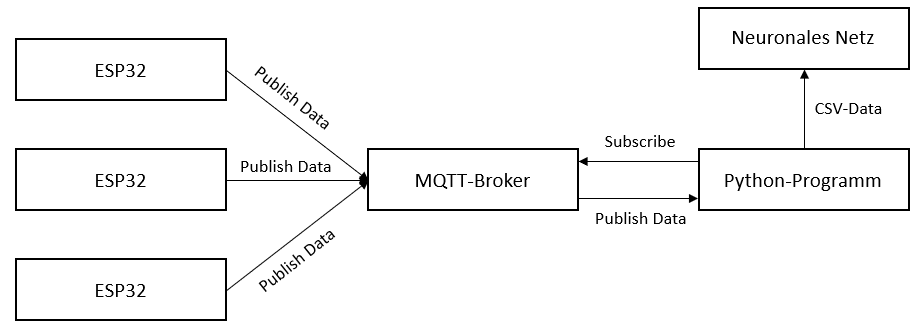
\includegraphics[width=0.9\textwidth]{images/com_arch.png}
	\caption{Die Kommunikationsarchitektur ohne Endgerät als Beispiel}
	\label{fig:com_arch}
\end{figure}
\newline
Das Python-Programm, welches die Daten in einer CSV-Datei speichert, published die Ergebnisse des neuronalen Netzes. Diese Ergebnisse nutzen die smarten Geräte als Steuerung. Abbildung \ref{fig:com_arch} zeigt die Kommunikationsarchitektur ohne die Anbindung an ein smartes Endgerät, da diese Kommunikation noch nicht hergestellt wird. Da die Ergebnisse am Ende gepublished werden, ist die Kommunikation offen, um mit smarten Geräten oder Möbeln zu kommunizieren. Sollte das neuronale Netz weiterhin als eigene Komponenten agieren, so müssen die Ergebnisse auch dementsprechend darüber an den Broker mitgeteilt werden und nicht über das Python-Programm, welches die Sensordaten erfasst. Dies passiert erst, sobald das neuronale Netz vollständig korrekt klassifizieren kann.

\section{Gegenüberstellung eines neuronalen Netzes mit TensorFlow und Numpy}
Um ein neuronales Netz zu programmieren gibt es verschiedene Möglichkeiten. In diesem Kapitel wird die Umsetzung mit der Numpy-Bibliothek und TensorFlow diskutiert. Die entsprechende Umsetzung beider Möglichkeiten findet in Kapitel \ref{sec:ums_nn} statt. Da in dieser Arbeit beide Möglichkeiten umgesetzt wurden, befinden sich auch entsprechend beide Erläuterungen im genannten Kapitel.
\newline
\newline
Da Numpy schon eine integrierte Standardbibliothek in Python ist, muss man sich keine weiteren Gedanken machen, eine externe Bibliothek in Python einzubinden. Der Aufbau eines neuronalen Netzes mit dieser Bibliothek muss komplett selbst gestaltet und entwickelt werden. So müssen also Aktivitätsfunktionen, Feedforward- und Backpropagation-Schritte erstellt werden, welche nicht aus der Bibliothek wie in TensorFlow bzw. Keras zur komfortableren Entwicklung mit entsprechenden Funktionen schon enthalten sind. Daher besteht der Vorteil mit TensorFlow unterschiedliche Kombinationen für ein neuronales Netz schneller Umsetzen und Ausprobieren zu können.
\newline
Wird bei der Entwicklung nur Numpy verwendet, lässt sich die sigmoid-Funktion zum Beispiel einfach Umsetzen, da Numpy eine mathematische Bibliothek von Python ist. Anders als mit Keras, bei der im entsprechenden Layer einfach der Name der Aktivitätsfunktion angegeben werden kann. Durch die mathematischen Vorteile mit Numpy kann ein einfaches neuronales Netz sehr simpel aufgebaut werden. Durch die einfache Umsetzung eines simplen neuronalen Netzes mit Numpy hat sich der Autor zu Beginn erst dafür entschieden, weil TensorFlow zu Beginn der Bachelorarbeit zu mächtig für kleine neuronale Netze ist und Keras dafür dem Autor nicht bekannt war. Weiterhin ist bei der Einschätzung aufgefallen, dass TensorFlow eher für Deep Neural Networks geeignet ist. Also für neuronale Netze mit mehr als zwei Hidden-Layer. Da das neuronale Netz nicht die gewünschten Ergebnisse liefert und zu einfach für die Anforderungen gestaltet ist, ist ein Umstieg auf die Einbindung von Keras als Frontend-Engine mit TensorFlow als Backend-Engine von Vorteil. Durch den Umstieg ist es möglich, einfach Layer hinzuzufügen und besser entscheiden zu können, welche Daten aus den Datensätzen für das Training und für den Test benutzt werden. Um einfach kleinere Netze zu programmieren reicht es aus, Numpy für die Umsetzung zu verwenden und Keras für Netze, die größer sind.

\section{Zusammenfassung und Ausblick}
Mit der beschriebenen Architektur zum Prototypen und dem neuronalen Netz möchte der Autor zeigen, dass es möglich ist, die Anforderungen und das Ziel aus Kapitel \ref{sec:goal} zum Prototypen umzusetzen. Des weiteren besteht damit die Möglichkeit dieses Gesamtsystem über den Prototypen hinaus weiterzuentwickeln, um diesen als finale Steuerung in ein Smart Home einzubinden. 
\newline
Die Gegenüberstellung der Architektur aus dem Praxisprojekt zum System in der Bachelorarbeit, zeigt, dass es besser ist einen Prototypen zu verwenden, welcher eine Komponente pro Sitzplatz auf dem Sofa verwendet. So ist es möglich, ein Sofa als Steuerung in größerem Umfang zu nutzen, wenn z.B. die Steuerung abhängig von der Sitzplatzzahl auf dem Sofa ist. Zusätzlich ist es mit dem Prototyp auch möglich, dass mehrere Personen gleichzeitig auf dem Sofa sitzen können und dies als Klassifizierung hinzu genommen werden kann. Dies wird allerdings nicht vom neuronalen Netz in dieser Arbeit mit einbezogen. Das zeigt die Möglichkeiten, welche in Zukunft implementiert werden können. So ist es wichtig, dass die Sensoren nicht beim Einbau in einem Sofa auffallen. Die Anzahl oder Größe der Sensoren spielt auch eine Rolle, damit der Nutzer das Sofa in vollem Umfang zur Steuerung benutzen kann. Daher sollte bei der Auswahl der Sensoren die Größe der jeweils zu messenden Fläche beachtet werden.
\newline
Beim neuronalen Netz ist es von Vorteil bei größeren Umsetzungen auf Bibliotheken wie TensorFlow zurückzugreifen. Für einfache Netze reicht Numpy aus, da man dort individuell ohne Bindung an Funktionen, die nicht unbedingt die gewünschten Ergebnisse bringen, die Umsetzung realisieren kann.
\newline
Wenn TensorFlow und Keras genutzt wird, können sehr einfach und schnell große neuronale Netze realisiert werden. Dies zeigt auch \citep{frochte2018} bei der Umsetzung eines neuronalen Netzes mit Keras und TensorFlow. In Zukunft ist es wichtig, dass die Sensoren weiter angepasst werden. Zusätzliche Klassifizierungen erweitern dann auch die Interaktionsmöglichkeiten mit dem Sofaprototypen.
\newpage
\chapter{Umsetzung des neuronalen Netzes zur Erkennung von Interaktionen}
Im Rahmen des Praxisprojekts entstand ein Prototyp, welcher ein Sofa darstellt, dass als Steuerung für smarte Endgeräte dient. Verwaltet wird das ganze von einem Regelsystem, welches nun durch ein neuronales Netz werden soll. Das aktuelle Kapitel erläutert die Umsetzung von der Aufgabe eines neuronalen Netzes im Smart Home bis zu den Funktionen des neuronalen Netz zur Verwaltung der Interaktionen.

\section{Umsetzung des neuronalen Netzes in Python}
\label{sec:ums_nn}
Das folgende Kapitel beschreibt die Umsetzung des neuronalen Netzes ohne eine Machine Learning Bibliothek und mit einer Bibliothek. Die Vorgehensweise eine Python-Bibliothek für Machine Learning zu nutzen, ist erst nach der Datensammlung mit verschiedenen Probanden kam erst als spätere Erkenntnis. Da der Datensatz sehr groß ist und die Nutzung einer schon vorhanden Bibliothek daher ein Vorteil ist um einfache Änderungen zur besseren Vorhersage vornehmen zu können.

\subsection{Umsetzung des neuronalen Netzes mit Numpy}
Zu Beginn dieser Umsetzung wurde eine Funktion geschrieben, welche die sigmoid-Funktion beinhaltet. Diese wird in einer Trainingsfunktion aufgerufen. Die Trainingsfunktion ist der Hauptteil dieses neuronalen Netzes. 
\newline
Die nachfolgende Erklärung des Python Codes beschreibt die Vorhersage mit einer Unit im output-Layer. Das komplette selbstgeschriebene neuronale Netz hat insgesamt drei Inputwerte und drei Outputwerte.
\begin{python}
def train():
    with open("values.txt") as f:
        dataset = [[int(x) for x in line.split(",")] 
                    for line in f]
        print(dataset)
\end{python}
Als erstes gilt in dieser Funktion das zusammen rechnen der Inputreize mit den Gewichtungen und die daraus errechnete Summe für jede Unit. An dieser Stelle bekommt das neuronale Netz jeweils drei Inputwerte pro Unit im Inputlayer.
\begin{python}
x = point[0] * w1 + point[1] * w2 + point[2] * w3 + b1
\end{python}
Ist die Summe ausgerechnet, dann werden die Ergebnisse in die Sigmoid Funktion übergeben und somit wird die Aktivierungsfunktion ausgelöst.
\begin{python}
pred1 = sigmoid(x)
\end{python}
Anschließend rechnet die Fehlerfunktion aus den Ergebnissen und dem gewünschten Ergebnis den mittleren quadratischen Fehler aus. Die Variable \(target\) beschreibt das gewünschte Ergebnis.
\begin{python}
cost1 = np.square(pred1 - target1)
\end{python}
Das Ergebnis dieser Fehlerfunktion zeigt also die Fehlerrate für die Vorhersagen mit den unveränderten Gewichtungen an. Als nächstes wird die Fehlerfunktion und sigmoid-Funktion abgeleitet.
Das \(d\) steht im Code für Derieved also abgeleitet. 
\begin{python}
dcost_dpred1 = 2 * (pred1 - target1)
dpred_dz1 = sigmoid_p(x)
\end{python}
Diese beiden Funktionen müssen nun nachfolgend multipliziert werden. Die dadurch entstehenden Ergebnisse müssen dann wieder durch multiplizieren mit dem gewünschten Ergebnis zusammen gerechnet werden. 
Um nun die Gewichte anzupassen, subtrahiert man das Gewicht mit der Lernrate und multipliziert diese mit den zuvor errechneten Kosten.
\begin{python}
dcost_dz1 = dcost_dpred1 * dpred_dz1
dcost_dw1 = dcost_dz1 * dz_dw1
w1 = w1 - learning_rate * dcost_dw1
\end{python}
Als weitere Erläuterung des Codes wird noch hinzugefügt, dass dieser Vorgang insgesamt 1000 Mal durchgeführt wird und die Lernrate beträgt 0,1.
\newline
Für sehr kleine und einfach gehaltene neuronale Netze kann dieses neuronale Netz verwendet werden. Da für das System aber acht Inputwerte genommen werden, müssten dementsprechend auch acht Gewichte benutzt und angepasst werden.

\subsection{Umsetzung des neuronalen Netzes mit Keras}
Das neuronale Netz bedient sich zur Umsetzung dem Frontend Keras. Dies ist eine unterstützte Bibliothek von Tensorflow. Tensorflow ist das backend und damit führt Keras alle Berechnungen und Vorhersagen durch. Da Keras eine Bibliothek für Python ist, ist das neuronale Netz auch entsprechende damit umgesetzt.
\newline
Als Ergänzung zu der Erklärung aus den Grundlagen \ref{sec:NNK} ist noch erweitert zu erläutern, dass das neuronale Netz zum Training in diesem Projekt Datensätze aus einer CSV-Dateien einliest. Die Testdaten werden aus dem Dataset als zufällige Anzahl ausgewählt. 
\newline
Das Fully-connected Neural Network ist untereinander mit allen Schichten verbunden. Zu Beginn muss ein Sequential Objekt in Python deklariert werden, damit das neuronale Netz Schicht für Schicht aufgebaut werden kann. Als Aktivierungsfunktion der Input Layers wird die ReLU-Funktion (Rectifier Linear Unit) benutzt. Bei dieser Funktion werden Ergebnisse kleiner null mit null ausgegeben und alles darüber mit dem Ergebnis, welches größer null ist. Die Aktivierungsfunktion des Output Layers ist die sigmoid Funktion. Als Fehlerfunktion wird Mean Squared Error verwendet und Adam als optimizer.
\newline
Aus den versuchen heraus die Fehlerrate zu gering wie möglich zu halten, ist der mittlere quadratische Fehler und die learning rate von 0,001 die beste Wahl.
Die Umsetzung des neuronalen Netzes ist aus einer Vorlage aus dem Buch \citep{frochte2018} entnommen und auf den Trainingsdatensatz vom Sofaprototypen angepasst.


\begin{figure}[H]
	\centering
		%[natürliche Breite in Pixeln, natürliche Höhe in Pixeln, Abhängigkeit von der Textbreite]
		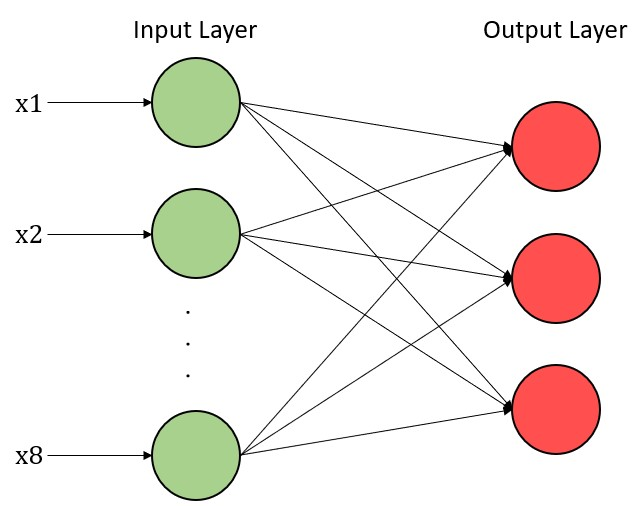
\includegraphics[width=0.6\textwidth]{images/NN.jpg}
	\caption{Darstellung des neuronalen Netzes zur Verwaltung der Interaktionen}
	\label{fig:NN}
\end{figure}

\section{Automatische Erkennung von Interaktionen}
Die Erkennung von Interaktionen findet über die Klassifizierung des neuronalen Netzes statt. Anhand der Ergebnisse aus dem feed forward Schritt und der darauf folgenden Backpropagation findet das neuronale Netz heraus, wie der Nutzer mit dem Sofa interagiert. 
\newline
Kann das neuronale Netz die Vorhersage richtig ausgeben, wird es als Künstliche Intelligenz in den Prototypen aufgenommen. Damit wird dann automatisch erkannt ohne weiteren Einfluss vom Nutzer, welches Gerät gesteuert werden muss.

\section{Neue Funktionen durch das neuronale Netz}
Die Hauptmerkmale zur Erkennung der Interaktionen verändern sich nicht mit dem neuronalen Netz. Das Regelsystem bestimmt anhand der Werte der Sensoren, welche Position der Nutzer auf dem Sofa einnimmt. Dies funktioniert aber nur, wenn die Personen immer für die Positionen die gleichen Sensoren besetzen. So muss für die Sitzposition immer die gleiche Position auf dem Sofa eingenommen werden. Dies ändert sich mit dem neuronalen Netz. Durch die Trainingsdaten wird im neuronalen Netz immer eingelesen wann eine Person sitzt, egal wie sie auf dem Sofa sitzt. Das hat den Effekt, dass jede Person selber entscheiden kann, wie sie sich auf das Sofa setzen möchte. Dadurch kann trotzdem immer das gleiche Endgerät aktiviert werden. Zudem muss bei neuen Liegepositionen und Sitzpositionen keine neue Regel hinzugefügt werden, da das neuronale Netz dies auch erkennent.
\newline
Für die Liegepositionen werden mit dem Regelsystem auch eigene Sensoren verwendet, damit unterschieden werden kann, was auf dem FSR und was mit FlexSensor passiert. Das neuronale Netz kann durch das Training erkennen, wann eine Person mit dem FSR interagiert und sitzt oder liegt. Also wird auf den Sitzkissen nur noch ein Sensor benötigt. Zudem ist es mit FlexSensoren sehr schwer zu erkennen, wann eine Person mit ihm interagiert, da dieser erst den Widerstand ab einer 45 Grad Biegung messen kann.

\newpage
\chapter{Evaluation des Trainings durch Probanden}
Mit der Evaluation wird die Auswertung der empirischen Methode zur Erfassung der Interaktionen mit dem Sofa erläutert. Weiterhin möchte der Autor die Ergebnisse und Erkenntnisse des neuronalen Netzes und des Gesamtsystems zeigen. Zudem finden in den folgenden Kapiteln auch die Beschreibungen des Aufbaus vom Prototypen auf einem realen Sofa statt. Der Autor möchte also eine Zusammenfassung der Ergebnisse und der empirischen Methode veranschaulichen, um daraus in Teil Sechs der Bachelorarbeit ein Fazit zu ziehen.

\section{Umgebung zur Erkennung von Interaktionen}
\label{sec:er_in}
Der Prototyp ist so aufgebaut, dass er beliebig um Sitzflächen auf einem Sofa erweitert werden kann. Für die empirische Methode wurde sich dafür entschieden, die Anzahl auf drei Sitzplätze zu beschränken. So kann das Sofa aus Abbildung \ref{fig:prot} benutzt werden. Jede zusammengesetzte Komponente aus Sensoren am ESP32 steht für einen Platz auf dem Sofa. Zwei ESPs haben einen FSR-Sensor mehr, da diese an den äußeren Sitzplätzen mit einer Armlehne ausgestattet sind. Für den akutellen Prototypen ist es nicht wichtig in welchem Raum, welche Möbel zusätzlich und welche Geräte vorhanden sind. Außerdem gibt es zwei unterschiedlich große FSR-Sensoren, die die gleichen Messwerte liefern und somit keine unterschiedliche Auswirkung auf die Sensorwerte im Datensatz haben.
\newline
\begin{figure}[H]
	\centering
		%[natürliche Breite in Pixeln, natürliche Höhe in Pixeln, Abhängigkeit von der Textbreite]
		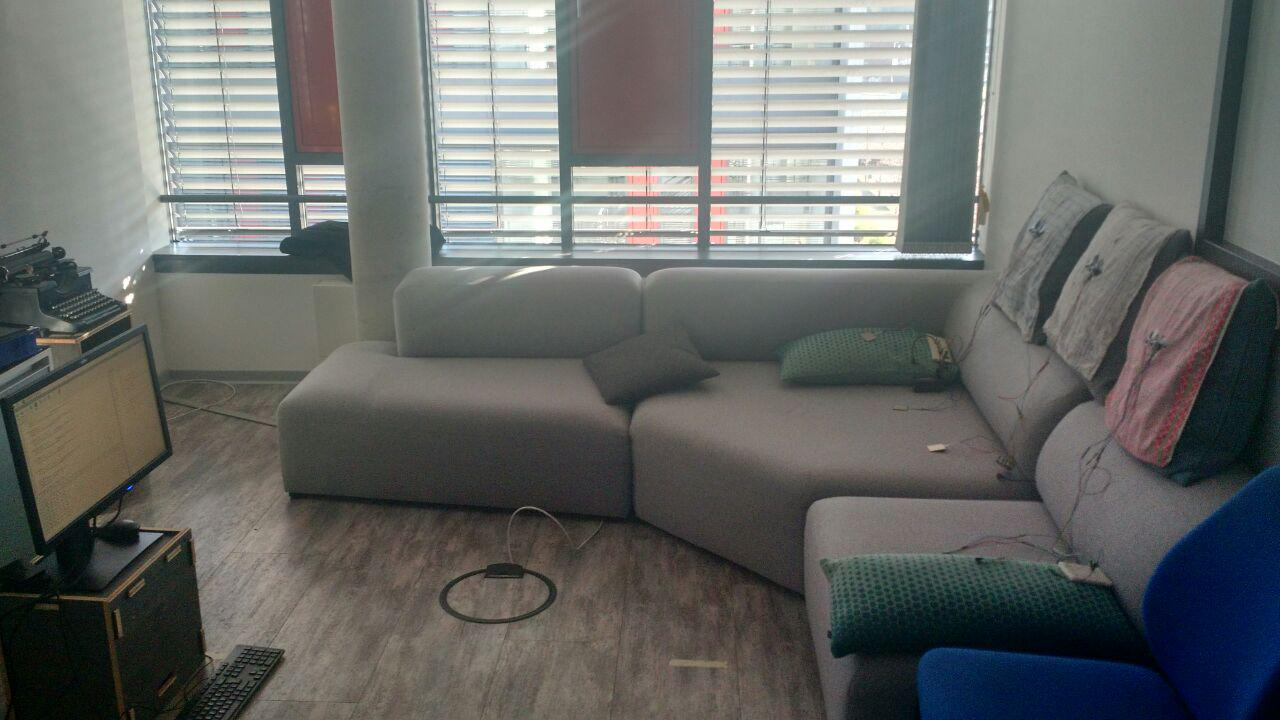
\includegraphics[width=0.75\textwidth]{images/prototyp.jpg}
	\caption{Realer Aufbau des Prototyps}
	\label{fig:prot}
\end{figure}

Abbildung \ref{fig:prot} zeigt den Prototypen, welcher auf einem Sofa aufgebaut ist. Die beiden grünen äußeren Kissen stellen die Armlehnen dar. Das wird gemacht, da dieses Sofa keine Armlehnen angebaut hat. Da der Prototyp für ein drei Personen Sofa ausgelegt ist, werden die Sitzplätze durch drei oben liegende Kissen getrennt. Auf der linken Seite ist der Raspberry Pi, mit dem darauf ausgeführten MQTT-Broker und Python-Programm zur Erfassung der Sensorwerte. Die Abbildung macht sichtbar, dass die Verwendung von Ultrasonic-Sensoren nicht positiv ist. Man kann also zum Schluss kommen, dass statt Ultrasonic-Sensoren, dünnere Sensoren die weniger auffallen, eingebaut werden müssen. Wenn Ultrasonic-Sensoren verwendet werdeb, dann muss immer eine Fläche in den Sofalehnen zusätzlich frei sein. Der Sensor kann dann dementsprechend den Abstand messen und der Nutzer muss sich immer im Radius der Wellen zur Messung des Abstands an die Rückenlehne anlehnen. Eine Möglichkeit zur Lösung des Problems kann durch Austauschen der Ultrasonic-Sensoren erfolgen, indem Sensoren verwendet werden, welche mehr Platz von der Rückenlehen einnehmen. Alternativ können mehrere kleine Sensoren verwendet werden.

\section{Soll-Ablauf der Situation}
\label{sec:abl}
Dieses Kapitel befasst sich mit der Beschreibung eines Ablaufs zur Sammlung der Daten indem die Probanden mit dem Sofa interagieren. Die folgende Beschreibung der Vorgehensweise zeigt, wie ein Proband in der Theorie mit dem Sofa interagiert, um die bestmögliche Erfassung der Sensordaten zu bekommen.
\newline
\newline
Um die Klassifizierung richtig vorhersehen zu können, erstellen Probanden durch Interaktionen mit Sofa einen Datensatz für die Trainings- und die Testphase wie sie in Kapitel \ref{subsec:eval} beschrieben ist. Ein Proband befindet sich immer alleine im Raum mit dem Sofa. So kann kein anderer Proband durch seine Interaktionen beeinflusst werden. Dort nimmt er verschiedene Positionen auf dem Sofa ein. Hat dieser seine Position festgelegt, werden die Sensorwerte in die CSV-Datei hinzugefügt. Die Position muss immer eine andere sein, damit die Variation mit den Sensoren sich so oft wie möglich unterscheidet. Der Proband soll sich immer hinlegen, hinsetzen oder das Sofa leer lassen. Der Ablauf ist mit jedem Probanden gleich und unterscheidet sich nur von den Interaktionen auf dem Sofa. Sobald 12 bis 15 Probanden diese Situation absolviert haben, wird das neuronale Netz mit diesem Datensatz trainiert und angepasst.
Die Probanden sehen außerdem auf dem Monitor, welche Position sie eingenommen haben in Form von den Sensordaten durch die Sensoren die sie benutzen.
\newline
Durch das Sammeln der Daten für den Datensatz soll außerdem getestet werden, wie die Probanden mit dem Sofaprotoypen umgehen und wie diese damit zurechtkommen. So wird dann gezeigt, welche Änderungen an dem Prototypen vorgenommen werden müssen, damit die Probanden die bestmögliche Interaktion mit dem Sofa ausführen können.

\newpage

\section{Tatsächlicher Ablauf aller Probanden}
\label{sub:real}
Der Autor führt aus Kapitel \ref{sec:abl} an, wie eine Datensammlung in der Theorie mit einem Probanden ablaufen soll. Der tatsächliche Ablauf mit allen Probanden erweist sich aber als Differenz zur Theorie. Insgesamt wurden mit 17 Probanden Daten gesammelt. In manchen fällen befanden sich mehrere Probanden im Raum, was den Interaktionen geholfen hat. Denn nicht jeder Proband kann sich sofort vorstellen, was mit den Interaktionen auf dem Sofa gemeint ist.
\newline
Jeder Proband nimmt verschiedene Positionen ein und auch unterschiedlich viele, da verschiedene Interaktionen mehrfach auftreten. Je mehr Probanden mit dem Sofa interagieren, desto häufiger treten damit die gleichen Positionen auf. Die Anzahl an Positionen nimmt mit mehr Probanden über die Zeit ab. Damit alle Probanden die gleiche Situation haben, ändert sich der Raum und das Sofa nicht. So hat jeder Proband die gleichen Voraussetzungen. Für diese empirische Methode ist auch kein smartes Gerät oder Möbelstück vorhanden. Da hier nur Sensordaten erfasst werden und das neuronale Netz noch keine entsprechende Vorhersage machen kann die immer korrekt ist.
\newline
Teile des Prototyps müssen zwischen den Interaktionen der Probanden auch hin und wieder neu zusammen gebaut werden, da es passieren kann, dass beim Anlehnen an die jeweilige Rückenlehne ein Kabel von den Ultrasonic-Sensoren durch den Probanden ohne Absicht getrennt wird. Die FSR-Sensoren sind zum Großteil nicht davon betroffen, da die Interaktionen nicht so stark auf die Kabel einwirken wie bei den Ultrasonic-Sensoren. Abgesehen davon gibt es mit den Interaktionen keine weiteren Probleme, außer das nicht jeder Proband immer selbstständig weiß, welche Positionen er machen muss. Dies ist aber unwichtig, da es bei dieser Datensammlung auch darum geht zu Testen, welche Änderungen am Prototyp gemacht werden müssen, damit der Proband besser mit dem System zurecht kommt.

\section{Aufbau des Datensatzes}
\label{sec:dataset}
In diesem Kapitel soll gezeigt werden, wie die Sensordaten für die Trainings- und Testphase gespeichert werden. Eine Position des Probanden ist eine Liste, die als eine Zeile in einer CSV-Datei liegt. Eine weitere CSV-Datei enthält die Positionen, die dem neuronalen Netz mit eingegeben werden. Kapitel \ref{subsec:ergeb} diskutiert die Ergebnisse aus dem neuronalen Netz und welche Optimierungen im weiteren vorgenommen werden, um die Vorhersagen mit den Testdaten genauer darzustellen. Die Tabelle \ref{tab:tablearr} stellt in abwärtiger Reihenfolge die festen Positionen der Sensoren in einem Array dar. Das folgende Beispiel der Daten einer CSV-Datei, zeigt die Positionen als Beispiel.
\newpage
\[0, 0, 134, 0, 3095, 0, 0, 717\]  
\[4095, 4095, 426, 84, 417, 580, 41, 456\]
\[0, 718, 136, 80, 3102, 4095, 530, 0\]
\newline
Der erste Datensatz zeigt ein leeres Sofa, der zweite eine sitzende Person und der dritte auch, nur auf der anderen Seite des Sofas. Was also aus dem Aufbau zu erkennen ist, dass es wichtig ist wie auch bei dem Regelsystem, wie der Datensatz aufgebaut ist, da sowohl das Regelsystem als auch das neuronale Netz erkennen muss, welcher Wert zu welchem Sensor zugewiesen ist.

\begin{table}[H]
	\centering
	\caption[Aufbau eines Arrays des Datensatzes]{Aufbau eines Arrays des Datensatzes}
		\vspace{1.0em}	
	\begin{tabular}{| l | p{5cm} | l | }
		\hline
		\rowcolor[gray]{0.9}\textbf{Sensor} & \textbf{Beschreibung} & \textbf{Werte} \\
		\hline
		\hline
		Sitzkissen Links & Ein FSR-Sensor erkennt die Sitz- bzw. Liegeposition eines Nutzers & 0 bis maximal 4095\\
		\hline
		Armlehne Links & Der FSR-Sensor erkennt den Kopf, Arm oder Fuß eines Nutzers & 0 bis maximal 4095\\
		\hline
		Rückenlehne Links & Anhand des Abstands wird erkannt, ob ein Nutzer sich anlehnt & ca. 3000 bis maximal 0 \\
		\hline
		Sitzkissen Mitte & Ein FSR-Sensor erkennt die Sitz- bzw. Liegeposition eines Nutzers & 0 bis maximal 4095\\
		\hline
		Rückenlehne Mitte & Anhand des Abstands wird erkannt, ob ein Nutzer sich anlehnt & ca. 3000 bis maximal 0\\
		\hline
		Sitzkissen Rechts & Ein FSR-Sensor erkennt die Sitz- bzw. Liegeposition eines Nutzers & 0 bis maximal 4095\\
		\hline
		Armlehne Rechts & Der FSR-Sensor erkennt den Kopf, Arm oder Fuß eines Nutzers & 0 bis maximal 4095\\
		\hline
		Rückenlehne Rechts & Anhand des Abstands wird erkannt, ob ein Nutzer sich anlehnt & ca. 3000 bis maximal 0\\ 
		\hline
	\end{tabular}
	\label{tab:tablearr}
\end{table}
\newpage

\section{Ergebnisse der Datensammlung}
\label{sub:res}
Es lässt sich anhand der Ergebnisse aus der Datensammlung zeigen, dass die FSR-Sensoren auch Werte größer 0 ausgeben und unterhalb des Maximalwerts liegen. Obwohl die Probanden keinen direkten Druck auf diese ausüben. Daraus lässt sich schlussfolgern, dass das neuronale Netz auch diese Datenpunkte erkennen muss. Damit wird bezweckt, dass die Ergebnisse trotzdem zur richtigen Vorhersage beitragen. Um zu überprüfen wie die Datenpunkte sich auf die Klassifizierung auswirken, testet der Autor den Datensatz sowohl mit und ohne Filterung der Datenpunkte.
\newline
Weiterhin sei auch zu erwähnen, dass die Abstandserkennung durch die Ultrasonic-Sensoren bei geringen Abständen sehr genau arbeitet. Wenn sich ein Proband anlehnt kann es auch vorkommen, dass ein Kabel von einem Ultrasonic-Sensor entfernt wird. Tritt dieser Fall auf, wird in der Datensammlung der Wert 0 gespeichert. Da ein Kabel immer dann abgerissen wird, wenn ein Nutzer sich anlehnt, ist es also korrekt, dass der Sensor den Wert 0 übergibt. Mit diesen Ergebnissen steht es außer Frage, dass die Datensammlung für das neuronale Netz geeignet ist. 

\section{Ergebnisse und Evaluation des neuronalen Netzes}
\label{subsec:ergeb}
Die folgenden Kapitel sollen die Evaluation des neuronalen Netzes näher erläutern. Es werden die Datensätze analysiert und deren Ergebnisse präsentiert. Weiterhin sollen Erkenntnisse aus den Ergebnissen gezogen werden. Das Kapitel zeigt außerdem die Unterschiede des Datensatzes wenn dessen Datenpunkte gefiltert in die Vorhersage eingenommen werden und wie die Klassifizierung ohne die Filterung der Datenpunkte aussieht.
\newline
Für das neuronale Netz werden zwei verschiedene Datensätze benutzt. Die Datensätze entstehen aus den gleichen Rohdaten, zeigen aber unterschiedliche Ergebnisse. Als erstes werden die Daten der Probanden benutzt ohne, dass sie verändert wurden. Damit will der Autor zeigen, wie die Ergebnisse des neuronalen Netzes aussehen, wenn alle Datenpunkte gespeichert sind. Denn eine Position tritt mehrfach in der CSV-Datei hintereinander auf. Mit der Abbildung \ref{fig:w_streu} soll gezeigt werden, wie das Lernverhalten des neuronalen Netzes mit allen Datenpunkten ausfällt. Dies bedeutet, dass eine Position mehrfach in die CSV gespeichert wird und damit können bei einer Position geringe Veränderungen auftauchen. Mit der Abbildung \ref{fig:wo_streu} wird dementsprechend gezeigt, wie das Lernverhalten ohne das Filtern der Datenpunkte aussieht.

\subsection{Datensatz mit dem Filtern von Datenpunkten}
Als ersten Datensatz werden die Positionen der Probanden verwendet, dass sie einmal in das neuronale Netz eingelesen werden. Dies bedeutet, dass jeder Datensatz nicht mehrfach auftaucht und so Veränderungen bei einer Position nicht gespeichert werden. So fällt das mehrfache Auftreten der Positionen weg und damit sieht auch das Ergebnis anders aus. Die folgende Abbildung \ref{fig:wo_streu} zeigt das Lernverhalten des neuronalen Netzes mit den gefilterten Datenpunkten. Anhand dieser Abbildung, zeigt der Autor auch den Unterschied zum unveränderten Datensatz. 
\newpage
Die Fehlerrate beim ersten Datensatz liegt bei 0,16. Damit liegt das neuronale Netz zu 84\% richtig bei den Vorhersagen. Für das Training- und die Testphase werden insgesamt 245 Positionen beim Filtern der Datenpunkte von allen 17 Probanden gespeichert. Der Unterschied zum Datensatz mit allen Datenpunkten ist sehr groß, da dieser aus 2934 Datensätzen besteht.

\begin{figure}[H]
	\centering
		%[natürliche Breite in Pixeln, natürliche Höhe in Pixeln, Abhängigkeit von der Textbreite]
		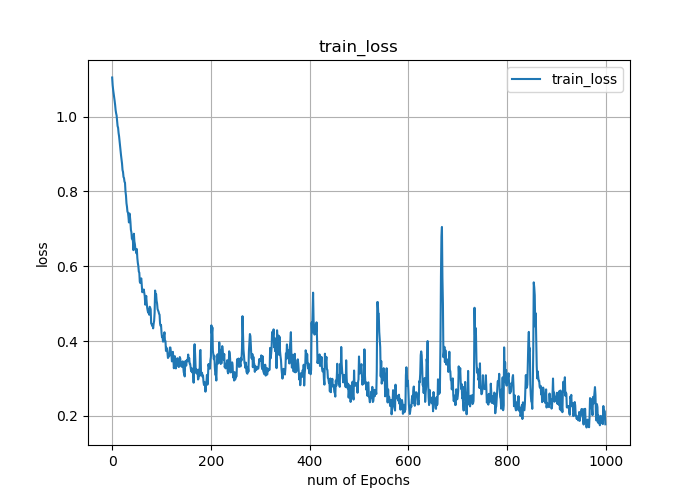
\includegraphics[width=0.7\textwidth]{images/wo_streu.png}
	\caption{Abbildung der Fehlerrate des neuronalen Netzes mit Filterung der Datenpunkte}	\label{fig:wo_streu}
\end{figure}

\subsection{Datensatz ohne Filterung der Datenpunkte}
\begin{figure}[H]
	\centering
		%[natürliche Breite in Pixeln, natürliche Höhe in Pixeln, Abhängigkeit von der Textbreite]
		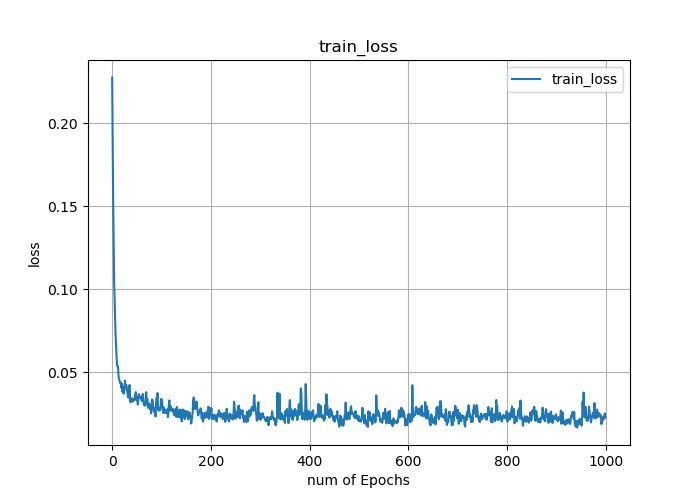
\includegraphics[width=0.7\textwidth]{images/w_streu_nn.png}
	\caption{Abbildung der Fehlerrate des neuronalen Netzes mit allen Datenpunkten}
	\label{fig:w_streu}
\end{figure}

Werden alle Datenpunkte in den Datensätzen gelassen, so liegt die Fehlerrate bei 0,03. Somit klassifiziert das neuronale Netz zu 99,7\% richtig. Damit ist es schon sehr nah an den 100\% und kann schon fast in den Prototypen mit eingebunden werden.

\section{Zusammenfassung der Evaluation}
Aus den vorherigen Kapiteln der Evaluation wird gezeigt, wie verschiedene Probanden mit dem Prototypen umgehen. So ist also nochmal zu sagen, dass der Prototyp durch ersetzen der Ultrasonic-Sensoren eine bessere Möglichkeit bietet um zu erkennen, wann ein Nutzer die Rückenlehne des Sofas verwendet. Wenn diese Sensoren ersetzt werden, kann die Rückenlehne des Sofas auch besser mit in die Verwaltung der Interaktionen einfliessen. 
\newline
\newline
Aus \ref{subsec:ergeb} ist zu erkennen, dass es besser ist ein neuronales Netz mit Daten zu trainieren, die so nah wie möglich an der Realität sind. Zudem verläuft das Training ohne die gefilterten Daten wesentlich besser ab. Es ist nicht wichtig wie viele Daten benutzt werden, sondern wie viele verschiedene Kombinationen dem neuronalen Netz zum trainieren gegeben wird. Durch die geringere Anzahl an Interaktionen die der Datensatz mit Filterung der Datenpunkte vorgibt, ist die Fehlerrate auch dementsprechend höher.

\section{Erkenntnisse aus der Evaluation zum Prototypen}
Aus folgender Überlegung aus dem Kapitel \ref{sub:real}, dass Probanden nach einer Zeit wiederholt die gleiche Sitzposition einnehmen, werden in diesem Kapitel die Schlüsse und Erkenntnisse daraus gezogen. Diese Erkenntnisse sind so beschrieben, dass bestimmte Punkte die Erkenntnis aus der Evaluation bilden.
\newline
So deuten diese Ergebnisse darauf hin, dass es von Vorteil ist, mehr Sensoren zur Erkennung der Interaktionen auf dem Sofa zu verbauen. So können weitere Werte aus den Realwerten gemessen werden, um so noch besser die Interaktionen im neuronalen Netz vorhersagen zu können. Als weitere Möglichkeit geht daraus hervor, nur FSR-Sensoren zu verwenden. Alternativ können auch Sensoren verwendet werden, welche die komplette Fläche einnehmen. Da die Probanden durch ihre Interaktionen auf dem Sofa Druck auf die Oberflächen ausüben, ist dies ein weiterer Grund nur FSR-Sensoren zu benutzen. Zusammengefasst kann also erwähnt werden, dass der Prototyp im aktuellen Zustand noch überarbeitet werden muss, da die Sensoren wie der Ultrasonic-Sensor für die Erkennung nicht von Vorteil ist. Also ist eine weitere Erkenntnis aus der Evaluation, dass für einen Prototypen mit dem Interaktionen aus Sitz- und Liegepositionen erfasst werden, Sensoren zu verwenden, welche ausschließlich den Druck oder die Kraft messen.
\newpage
Anhand des letzten Kapitels wird gezeigt wie Vorhersagen ausfallen, wenn ein Datensatz mit allen Datenpunkten verwendet wird. Zusätzlich wird der Datensatz aus den Sensorwerten erstellt bei dem die Position nur einmal gespeichert wird. Zusammengefasst liegt die Fehlerrate bei dem Datensatz mit den gefilterten Datenpunkten bei 0,16. Dies ist im Vergleich zur Fehlerrate von 0,03 eine großer Unterschied. Dies zeigt, dass das Trainieren mit allen Datenpunkten besser ist. 


\newpage
\chapter{Fazit und Aussicht für den Prototypen}

\section{Zusammenfassung der Bachelorarbeit}
\section{Zukunftsaussicht für das System}
\newpage
\chapter{Anhang}
\addtocontents{toc}{\protect\thispagestyle{empty}}

\begin{python}
import paho.mqtt.client as mqttClient
import time
import sys

sensors = [0, 0, 0, 0, 0, 0, 0, 0]
pubMsg = ""

def on_connect(client, userdata, flags, rc):

    if rc == 0:

        print("Connected to broker")

        global Connected                
        Connected = True                

    else:

        print("Connection failed")

def on_message(client, userdata, message):

    if message.topic == "fsr1":
        print("Message received 1: "  + 
               message.payload.decode("utf-8"))
        sensors[0] = message.payload.decode("utf-8")

    if message.topic == "fsr2":
        print("Message received 2: "  + 
               message.payload.decode("utf-8"))
        sensors[1] = message.payload.decode("utf-8")

    if message.topic == "dis":
        print("Message received 3: "  + 
               message.payload.decode("utf-8"))
        sensors[2] = message.payload.decode("utf-8")

    if message.topic == "fsr3":
        print("Message received 4: "  + 
               message.payload.decode("utf-8"))
        sensors[3] = message.payload.decode("utf-8")

    if message.topic == "dist2":
        print("Message received 5: "  + 
               message.payload.decode("utf-8"))
        sensors[4] = message.payload.decode("utf-8")

    if message.topic == "fsr4":
        print("Message received 6: "  +
               message.payload.decode("utf-8")
        sensors[5] = message.payload.decode("utf-8")

    if message.topic == "fsr5":
        print("Message received 7: "  + 
               message.payload.decode("utf-8"))
        sensors[6] = message.payload.decode("utf-8")


    if message.topic == "dist3":
        print("Message received 8: "  + 
               message.payload.decode("utf-8"))
        sensors[7] = message.payload.decode("utf-8")

    print(sensors)
    file2write=open("dataset.txt",'a')
    file2write.write(str(sensors) + "\n")
    file2write.close()

def on_publish(client, userdata, result):
    print("Data published \n")
    pass

Connected = False

broker_adress = "IP Adress of the broker"
port=1883

client = mqttClient.Client("mosq/E4hpAcdlgjIy5b74cE")
client.on_connect= on_connect
client.on_message= on_message
client.connect(broker_adress, port=port)  
client.loop_start()

while Connected != True:    
    time.sleep(0.1)

client.subscribe("fsr1")
client.subscribe("fsr2")
client.subscribe("fsr3")
client.subscribe("fsr4")
client.subscribe("fsr5")
client.subscribe("dis")
client.subscribe("dist2")
client.subscribe("dist3")

try:
    while True:
        time.sleep(1)

except KeyboardInterrupt:
    print("exiting")
    client.disconnect()
    client.loop_stop()

client1 = mqttClient.Client("controller1")
client1.on_publish = on_publish
client1.connect(broker_adress, port=port)
ret = client.publish("living_room", pubMsg)
\end{python}

\newpage

\begin{python}

\end{python}

\newpage


\newpage
%Erzeugt ein Abbildungsverzeichnis
	\listoffigures
	%Fügt die Zeile "`Abbildungsverzeichnis"' als Chapter ins Inhaltsverzeichnis ein
	\addcontentsline{toc}{chapter}{Abbildungsverzeichnis}
\newpage
	
	%Erzeugt ein Tabellenverzeichnis
	\listoftables
	%Fügt die Zeile "`Tabellenverzeichnis"' als Chapter ins Inhaltsverzeichnis ein
	\addcontentsline{toc}{chapter}{Tabellenverzeichnis}
\newpage

% To change the title from References to Bibliography:
\renewcommand\refname{Literaturverzeichnis}

%Paket für ein deutsches Literaturverzeichnis

\bibliographystyle{natdin} % or try natplain or unsrtnat
\bibliography{literatur} % refers to literatur.bib

	%Fügt die Zeile "`Literaturverzeichnis"' als Chapter ins Inhaltsverzeichnis ein
	\addcontentsline{toc}{chapter}{Literaturverzeichnis}
\newpage

%!TEX root = ../Masterthesis_Fischer.tex
\chapter*{Eidesstattliche Erklärung}
%\addcontentsline{toc}{chapter}{Eidesstattliche Erklärung}

Ich versichere, die von mir vorgelegte Arbeit selbständig verfasst zu haben.\\ \\
Alle Stellen, die wörtlich oder sinngemäß aus veröffentlichten oder nicht veröffentlichten Arbeiten anderer entnommen sind, habe ich als entnommen kenntlich gemacht. Sämtliche Quellen und Hilfsmittel, die ich für die Arbeit benutzt habe, sind angegeben.\\ \\
Die Arbeit hat mit gleichem Inhalt bzw. in wesentlichen Teilen noch keiner anderen Prüfungsbehörde vorgelegen.
\vspace{1.5cm}
\\
Gummersbach, \today
\vspace{0.2cm}
\begin{figure}[H]
	\hspace{-1cm}
		%[natürliche Breite in Pixeln, natürliche Höhe in Pixeln, Abhängigkeit von der Textbreite]
		
\includegraphics[width=0.4\textwidth]{images/unterschrift.png}
\end{figure}
\\
\hspace{-0.4cm}Jan Schröder


% chapter eidesstattliche_erklärung (end)



\end{document}